\subsection{Oblate spheroidal fluid particles}

Many studies have been conducted to determine the influence of the droplets' deformation on suspension Rheology \citet{goddard1967nonlinear,lhuillier1987phenomenology,maffettone1998equation}.
Most of the authors considered the Rheology of such an emulsion for neutrally buoyant droplets in linear flows. 
In this work, we would like to present a more general framework in which we consider the deformation of droplet's in arbitrary flows. 
In this section we first describe the behavior of a single deformable drop. 
Latter in this paper we present the influence of such a deformation on the suspension rheology. 
At this stage the only restriction that we make about the drop is that it possesses oblate spheroidal shape. 
This is consistent with shape that adopt buoyant droplets or bubbles rising in a Newtonian fluid. 

\subsubsection*{Shape description of the droplet}
We consider oblate spheroidal droplets as it is depicted \ref{fig:scheme_spheroid}. 
\begin{figure}[h!]
    \centering
    \hfill
    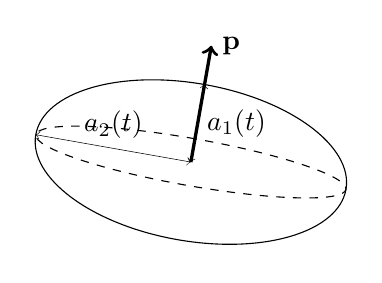
\begin{tikzpicture}[rotate=80]
        \draw(0,0) ellipse (1 cm and 2 cm);
        \draw[dashed](0,0) ellipse (0.3 cm and 2 cm);
        \draw[<->,very thin](0,0) --++ (1,0)node[midway,right]{$a_1(t)$};
        \draw[->,very thick](0,0) --++ (1.5,0)node[right]{$\textbf{p}$};
        \draw[<->,very thin](0,0) --++ (0,2)node[midway,above]{$a_2(t)$};
    \end{tikzpicture}
    \hfill
    \caption{Scheme of an  oblate spheroid oriented along the unit vector \textbf{p} with $a_1(t)$ and $a_2(t)$ the length of the semi axes of the spheroid.
    Note that when the drop is spherical we have $a_1=a_2=a$}
    \label{fig:scheme_spheroid}
\end{figure}
This shape might be described completely by the second moment of mass, $\textbf{M}_\alpha$.
In this context, each eigenvalue of the second moment of mass tensor is proportional to square semi axes of the particle. 
Indeed, by direct integration over the spheroidal particle volume we may find :
\begin{equation*}
    \textbf{M}_\alpha
    = \frac{m_\alpha a^2}{5}\left[
        \left(\frac{a_1}{a}\right)^2\textbf{pp}
        + \left(\frac{a_2}{a}\right)^2 (\textbf{I} - \textbf{pp}),
    \right] 
\end{equation*}
Additionally, note that due to the volume conservation condition we have : $ a_2^2 a_1 = a^3$. 
This means that : $M_1 = M_2^{-2}$, where the $M_i$ are the eigenvalues of the dimensionless tensor $\frac{m_\alpha a^2}{5}\textbf{M}_\alpha^* = \textbf{M}_\alpha$. 
Note that if we consider small deformations, meaning $M_1 - 1 \ll 1$ we have $M_1  = M_2^{-2} = 1 - 2 (M_2 - 1) + \mathcal{O}((M_2 -1)^2)$. 
Consequently, for small deformation the trace of the second moment of mass tensor reads :  $\frac{1}{3}\textbf{I}:\textbf{M}_\alpha = M_1 + 2M_2 = 1 - 2M_2 + 2M_2 = 1$. 
Therefore in the limit of small deformation the droplet shape is completely determined by one scalar value $M_1$ or $M_2$, and the orientation tensor $\textbf{p}$. 

Additionally, with this definition we can introduce the distance function  $\FF_\alpha$. 
It reads, 
\begin{equation*}
    \FF_\alpha(\textbf{x},t) = \textbf{rr}:\textbf{M}_\alpha^* -a^2.  
    \label{eq:distance_function}
\end{equation*}
The point on the surface of the particle are defined through $\FF_\alpha(\textbf{x}_I,t) = 0$. 
Being able to define the droplet's shape in such a rigorous way will find its use in the calculation of the surface tension stress. 
Using these definition makes the dimensionless  second moment of mass the same as the Cauchy green deformation tensor. 

\subsubsection*{The droplet's internal velocity}


We know that an isolated droplet in creeping flow with translating motion exhibit internal motion known as Hill vortexes, see \ref{fig:flowlines} (b). 
For a drop immersed in an unbounded linear flow, still in stokes flows, we can derive an analytical solution such that $\textbf{w}_2^0 \sim \textbf{rrr}$, see \ref{fig:flowlines} (a). 
If slightly more inertial effects are present one might find that the internal motion are close to hill's vortexes but with an overall oblate spheroidal shape, see \ref{fig:flowlines} (c). 
In these cases the droplet's internal velocity fields is a steady solution.
Nevertheless, for a droplet to go from case (b) to case (c) a deformation must occur. 

To account for this deformation in our case we assume that the secondary velocity field that is responsible for the deformation is purely a linear function of the position. 
The internal velocity field of a particle under homogeneous linear deformation can be described as such, $\textbf{w}_2^0 = \bm\Gamma_\alpha \cdot \textbf{r}$. 
We have introduced, $\bm\Gamma_\alpha$, the mean velocity gradient inside the particle, which symmetric part : $\textbf{E}_\alpha$, represents the rate of strain, and skew symmetric part : $\bm\Omega_\alpha$, represents the angular velocity. 

\begin{figure*}
    \centering
    \begin{tikzpicture}
        \node (img3) at (0.6\textwidth,0) {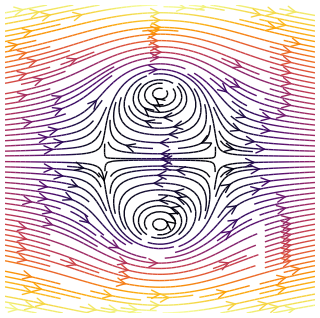
\includegraphics[width=0.3\textwidth,angle=270]{image/Rising_def_Stokes.png}};
        \node (img2) at (0.3\textwidth,0) {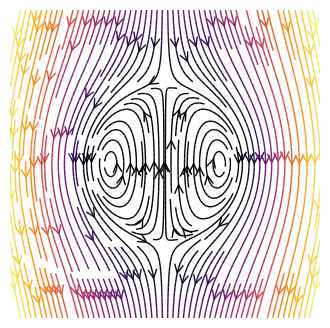
\includegraphics[width=0.3\textwidth]{image/Rising_Stokes.png}};
        % \draw (0.45\textwidth,0)node{$\rightarrow$};
        % \draw (0.45\textwidth,0.4cm)node{$\bm\Gamma_\alpha\cdot \textbf{r}$};
        \node (img1) at (0.0\textwidth,0) {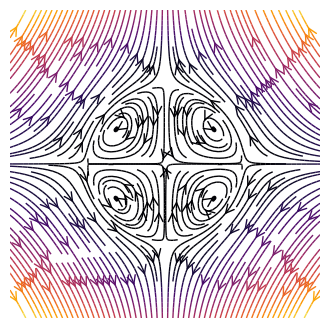
\includegraphics[width=0.3\textwidth]{image/Shear_Stokes.png}};
        \draw (img3.south)node{(c)};
        \draw (img2.south)node{(b)};
        \draw (img1.south)node{(a)};
    \end{tikzpicture}
    \caption{Three examples of steady state flow lines plots of an isolated droplet immersed into a viscous fluid. 
    (a) Rising sphere in uniform stokes flow (analytical solution in \ref{ap:Translating_sphere}). 
    (b) Fixed droplet in extensional flow (analytical solution in \ref{ap:Translating_sphere}).
    (c) Deformed droplet in rising motion (analytical solution of \citet{taylor1964deformation}). }
    \label{fig:flowlines}
\end{figure*}
To summarize, we assume that the inner velocity field of the drop can be decomposed into two distinct part. 
The first one is the steady state component, examples are : hill's vortex for spherical and oblate spheroidal drop in steady linear motion, the inner velocity field of a drop in steady linear flows, and so on. 
The second contribution is the inner velocity fields that alter the drop's shape, this field is assumed linear with the position and homogeneous, that is $\bm\Gamma\cdot \textbf{r}$. 
Adopting these definitions, the particle internal velocity is written, 
\begin{equation}
    \textbf{w}_{2,i}^0(\textbf{x}_\alpha)
    = \bm\Gamma_{\alpha,ik}(t) \cdot \textbf{r}_k
    + \textbf{w}^{s}_{2,i}(t,\textbf{r})
    =\bm{\Omega}_{\alpha,ik}\cdot \textbf{r}_k
    + \textbf{E}_{\alpha,ik} \cdot \textbf{r}_k
    + \textbf{w}^{s}_{2,i}(t,\textbf{r})
    \label{eq:def_vel}
\end{equation}
Where we introduced the vector $\textbf{w}^{s}_2(t,\textbf{r}) =\textbf{w}^{0}_{2,i}(t,\textbf{r})  - \bm\Gamma_{\alpha,ik}(t) \cdot \textbf{r}_k$ which represents all the internal motions that does not alter the drop's shape. 

An important consequence of this definition is that the integral on the RHS of \ref{eq:dt_S_alpha} is null when $\textbf{w}_{2,i}^0 = \textbf{w}_{2,i}^s$. 
This can be shown by re writting the second moment of mass equation with the use of the velocity decomposition.
This yields,
\begin{equation*}
    \ddt \textbf{M}_{\alpha,ik}
    = 
    \textbf{M}_{\alpha,ik} \cdot \bm\Gamma_{\alpha,kj}
    +  \bm\Gamma_{\alpha,ki} \cdot \textbf{M}_{\alpha,jk}
    +
    \intO{ 
        \textbf{w}_{2,i}^s\textbf{r}_j
        + \textbf{r}_i\textbf{w}_{2,j}^s
    }
\end{equation*}
In the cases where $\bm\Gamma = 0$, the droplet shape remains steady, in this case $\ddt \textbf{M}_\alpha = 0$ and $\intO{\textbf{w}^{s}_{2,i} \textbf{r}_j + \textbf{r}_i \textbf{w}_{2,i}^s} = 0$. 
In the case where $\bm\Gamma \neq 0$ the droplets deform according to the linear velocity fields $\bm\Gamma\cdot \textbf{r}$.
Since we assumed that no other source of deformation are present than the latter, we must have $\intO{\textbf{w}^{s}_{2,i} \textbf{r}_j + \textbf{r}_i \textbf{w}_{2,i}^s} = 0$ so that $\textbf{w}^{s}_{2,i} $ doesn't contribute to the deformation nor the rotation.
This, means that $\textbf{w}^{s}_{2,i}$ is a velocity fields determined in  part by the instantaneous shape of the droplet and its , that does not alter the shape of the drop. 
Additionally, the angular momentum is assumed to be entirely described by $\textbf{M}_\alpha \cdot \bm\Omega_\alpha$ meaning that, $\textbf{r} \textbf{w}_{2}^s$ plays no role at all in the total particle's moment of momentum.
This type of velocity fields is encountered in linear skew symmetric flows where the rotation is homogeneous and follow the carrier fluid vorticity. 
Anyhow, this velocity decomposition has the plaisent property that $\textbf{P}_\alpha = \bm\Gamma \cdot \textbf{M}_\alpha + \intO{\textbf{w}^{s}_{2,i} \textbf{r}_j} =  \bm\Gamma \cdot \textbf{M}_\alpha $ at all time, which will simplify the equaitons of motions. 

Now some constrain should apply on the tensor $\textbf{E}_\alpha$.
Indeed, the mass conservation inside the particle \ref{eq:dt_rho} impose $\div \textbf{u}_2^0 = \textbf{E}_\alpha : \textbf{I}= 0$, where it is assumed that $\div \textbf{w}_2^s =0$. 
Also, note that to preserve the spheroidal shape of the particle we must assume that the particle's rate of strain principal direction is the same as the droplet's shape principal axis. 
In other worlds, $\textbf{E}_\alpha$ must have the same eigenbasis as $\textbf{M}_\alpha$. 
Making up with these two constrain leads to the expression : $\textbf{E}_\alpha = -2 E_2 \textbf{pp} + E_2 (\textbf{I}- \textbf{pp})$, where $E_2$ is the second eigenvalue of $\textbf{E}_\alpha$. 


As it is demonstrated in \ref{ap:Translating_sphere} the internal motion of an isolated spherical drop, such as the one in \ref{eq:def_vel}, is entirely determined  from $\textbf{u}_1$,$\grad\textbf{u}_1$,$\textbf{u}_\alpha$ and so on. 
Therefore, it is reasonable to think that in a more general case, $\textbf{w}_2^s$ might be entirely determined by the carrier fluid and particles' properties, namely, $\textbf{u}_\alpha$ $\textbf{M}_\alpha$, $\textbf{u}_1$ $\grad\textbf{u}_1$ and for non-dilute flows we might have $\phi_2$ or more complicated functions. 
Thus, from now on we consider that the internal velocity $\textbf{w}^{s}_2(t,\textbf{r})$ is not part of the particle' unknown, but rather is a closure term. 
Consequently, in this problem a single droplet is described exhaustively by, $\textbf{x}_\alpha, \textbf{u}_\alpha, \textbf{M}_\alpha$ and $\bm\Gamma_\alpha$. 
This requires two additional equations one for $\textbf{M}_\alpha$ and another for $\bm\Gamma_\alpha$. 

\subsubsection*{The conservation equations}

The integrals appearing in \ref{eq:dt_M_alpha} and \ref{eq:dt_P_alpha} can be reformulated using the previous decomposition of the internal velocity field, and it reads, 
\begin{align}
    \intO{(\textbf{rw}_ 2^0 )_{ij}+ (\textbf{w}_2^0 \textbf{r})_{ij}} 
    = \textbf{M}_{\alpha,ik} \cdot \bm\Gamma_{\alpha,jk}
        +  \bm\Gamma_{\alpha,ik} \cdot \textbf{M}_{\alpha,jk}
    \\
    \intO{\rho_2 \textbf{w}_{2,i}^0\textbf{w}_{2,j}^0}
    = \bm\Gamma_{\alpha,jl}\bm\Gamma_{\alpha,ik} \textbf{M}_{\alpha,kl}  
        +\intO{\rho_2 \textbf{w}_{2,i}^s\textbf{w}_{2,j}^s}
    \\
    \intO{\bm\sigma_{2,ij}^0}
    =
    2 \mu_2 v_\alpha \textbf{E}_{\alpha,ij}
    - \intO{p_2^0} \textbf{I}_{ij}
    + \mu_2 \intS{(\textbf{n}_i \textbf{w}_{2,j}^s + \textbf{n}_j \textbf{w}_{2,i}^s)}
    \\
    \intS{\bm\sigma_{I,ij}^0}
    = \frac{\gamma v_\alpha }{a} \left[
        2\textbf{I}_{ij} 
        - \frac{4  }{5} (\textbf{M}_{\alpha,ij}^* - \textbf{I}_{\alpha,ij})
    \right]
    +\mathcal(O)((\textbf{M}_\alpha-\textbf{I})^2)\\
    % s_\alpha 
    % = 4\pi a^2 (1+\frac{\textbf{M}:\textbf{M}}{15})
\end{align}
The reformulation of the moment of momentum have already been treated above. 
The surface tension stress has been derived in the limit of small deformation. 
Note that our formula agree with the one derived by \citet{lhuillier1987phenomenology}. 
The detailed calculation of the surface tension stress tensor is given in appendix. 
We provide the exact results as well as the Taylor expansion of this formula for small deformation. 

Injecting these formulas inside \ref{eq:dt_M_alpha} and \ref{eq:dt_P_alpha} yields an equation for the deformation and the rate of strain of the drop. 
If we separate the skew-symmetric, symmetric and trace of the moment of momentum equation we obtain and equation for $\bm\Omega_\alpha$ and one fer  $\textbf E_\alpha$, namely,
\begin{align*}
    % \ddt \textbf{pp}_{\alpha,ij}
    % = \textbf{pp}_{\alpha,ik} \cdot \bm\Omega_{\alpha,jk}
    % +  \bm\Omega_{\alpha,ik} \cdot \textbf{pp}_{\alpha,jk}\\
    \ddt \textbf{M}_{\alpha,ij}
    = \textbf{M}_{\alpha,ik} \cdot \bm\Gamma_{\alpha,jk}
    +  \bm\Gamma_{\alpha,ik} \cdot \textbf{M}_{\alpha,jk}\\
    \ddt (\textbf{I}_{\alpha,ik}\bm\omega_{\alpha,k} )
    = 
    \intS{(\textbf{r}\times\bm\sigma_1^0\cdot \textbf{n})_i} \\
    \frac{1}{2}\ddt^2 \textbf{M}_{\alpha,ij}
    -  \bm\Gamma_{\alpha,jl}\bm\Gamma_{\alpha,ik} \textbf{M}_{\alpha,kl}  
    + \mu_2 v_\alpha 2\textbf{E}_{\alpha,ij}
    + \frac{\gamma v_\alpha }{a} \left[
    2\textbf{I}_{ij} 
    - \frac{4 }{5} (\textbf{M}_{\alpha,ij}^* - \textbf{I}_{\alpha,ij})
    \right]\\
    = 
    \frac{1}{2}\intS{(\textbf{r}\bm\sigma_1^0 + \bm\sigma_1^0\textbf{r})\cdot \textbf{n}} 
    + \intO{\rho_2 \textbf{w}_{2,i}^s\textbf{w}_{2,j}^s}
    + \intO{p_2^0} \textbf{I}_{ij}
    - \mu_2 \intS{(\textbf{n}_i \textbf{w}_{2,j}^s + \textbf{n}_j \textbf{w}_{2,i}^s)}\\
    % \frac{1}{2}\ddt^2 \textbf{M}_{\alpha,mm}
    % -  \bm\Gamma_{\alpha,ml}\bm\Gamma_{\alpha,mk} \textbf{M}_{\alpha,kl}  
    % + \frac{\gamma v_\alpha }{a} 
    % \left[
    % 2\textbf{I}_{mm} 
    % % - \frac{4 }{5 } (\textbf{M}_{\alpha,mm}^* - \textbf{I}_{\alpha,mm})
    % \right]
    % = 
    % \intS{\textbf{r}_m\cdot\bm\sigma_{1,mk}^0\cdot \textbf{n}_k} 
    % + \intO{\rho_2 \textbf{w}_{2,m}^s\cdot \textbf{w}_{2,m}^s}
    % + \intO{p_2^0} \textbf{I}_{mm}
\end{align*}
The second moment of mass \ref{eq:dt_Cs}, is consistent with the equation found by \citet{goddard1967nonlinear} and \citet{lhuillier1987phenomenology}. 
Following, \citet{goddard1967nonlinear}  terminology, the left-hand side of \ref{eq:dt_Cs} is referred as the \textit{convected} derivative of $\textbf{M}^*_\alpha$. 
Therefore, the \textit{convected} derivative of $\textbf{M}_\alpha$ is equal to the rate of strain of the particle. 
The skew-symmetric part of the first moment of momentum \ref{eq:dt2_C}, it is basically the angular momentum balance of a non-spherical object. 
The right-hands side accounting for the external torque contribution. 
The symmetric part however has the form of a non-linear forced harmonic oscillatory equation for the droplet deformation. 
Indeed, the first groups of terms on the left-hand side represent the inertial contribution of the droplet internal fluid. 
It is made of a second order derivative plus non-linear terms in $\bm\Gamma_\alpha$. 
The second groups of terms is internal viscous contribution that arise directly from the definition of the stress \ref{eq:sigma_2_def}. 
It vanishes for small viscosity ration and is linear in the first derivative of $\textbf{M}_\alpha$. 
The last term on the left-hand side is the elastic response from the interface which is negligible for high capillary number $Ca \to \infty$. 
Then on right-hand side of the equation we find the first moment of surface force, $\intS{(\textbf{r}\bm\sigma_1^0+ \bm\sigma_1^0\textbf{r})\cdot \textbf{n}}^*$ which has an unknown expression at this stage. 
\ref{eq:dt2_C} might be regarded as a second order harmonic equation with non-linear contributions. 
However, the unknown integrals $\intO{\rho_2 \textbf{w}_{2,i}^s\textbf{w}_{2,j}^s},
\intS{(\textbf{n}_i \textbf{w}_{2,j}^s + \textbf{n}_j \textbf{w}_{2,i}^s)}$ and $\intS{(\textbf{r}\bm\sigma_1^0+ \bm\sigma_1^0\textbf{r})\cdot \textbf{n}}^*$ are in general function of the shape of the particle so on $\textbf{M}_\alpha$ and its higher derivatives of $\textbf{M}_\alpha$.
These terms have to be seen as forcing terms. 
Therefore, at this stage it is impossible to predict the nature of the harmonic regime followed by the droplet. 
To conclude on this matter one must find an expression for all this closure as well as determinate the impact of the non-linear terms.



We now focus on the rate of strain equation. 
To better understand this equation we introduce the following dimensionless groups, 
\begin{align*}
    \intO{\rho_2 \textbf{w}_{2,i}^0\textbf{w}_{2,j}^0}
    \sim \frac{m_\alpha a^2}{\tau_u^2} \textbf{F}_{ww}^*
    \\
    - \intO{p_2^0\textbf{I}}
    + \mu_2 \intS{(\textbf{n}_i \textbf{w}_{2,j}^s + \textbf{n}_j \textbf{w}_{2,i}^s)}
    \sim \frac{v_\alpha \mu_2}{\tau_u} \textbf{F}_{e}^*
    \\
    \intS{\textbf r \bm\sigma_1^0 \cdot \textbf{n}}
    \sim 
    \frac{v_\alpha \mu_1}{\tau_u} \textbf{F}_{\sigma}^*
\end{align*} 
where we have assumed that the internal and external stress contribution followed a viscous scaling. 
The time $\tau_u$ represent the external solicitation time-scale. 
Which is in opposition to the droplets rate of strain and rotation time scale such that $\bm\Gamma = 1/\tau \bm\Gamma^*$. 
\begin{align*}
    \frac{\zeta Re}{5}\left[
        \beta^2 \frac{1}{2}\ddt^2 \textbf{M}_{\alpha,ij}
    -   \beta^2 \bm\Gamma_{\alpha,jl}\bm\Gamma_{\alpha,ik} \textbf{M}_{\alpha,kl}  
    - \textbf{F}_{ww}^*
    \right]
    + \lambda  \left[
        \beta 2\textbf{E}_{\alpha,ij}
    +  \textbf{F}_\sigma^*
    \right]
    + \frac{1}{Ca} \left[
    2\textbf{I}_{ij} 
    - \frac{4  }{5} (\textbf{M}_{\alpha,ij}^* - \textbf{I}_{\alpha,ij})
    \right]
    = 
    \frac{1}{2}
    \textbf{F}_{\sigma_1}^*
    % \intS{(\textbf{r}\bm\sigma_1^0 + \bm\sigma_1^0\textbf{r})\cdot \textbf{n}} 
    % + \intO{p_2^0} \textbf{I}_{ij}
\end{align*}
where we have defined the following dimensionless groups : 
\begin{align*}
    \beta = \frac{\tau_u}{\tau}
    && \zeta = \rho_2 /\rho_1
    && \lambda = \mu_1/\mu_2 
    && Re = \frac{\rho_1 a^2 }{ \mu_1 \tau_u}
    && Ca = \frac{a \mu_1}{\gamma \tau_u}
\end{align*}

We now examine the specific case studied by \citet{lamb1924hydrodynamics} where he considered no external contribution around the particle nor rotational motion.
Also, it is considered that the deformation within the particle are linear and small. 
Keeping only the trace of this equation yields the low deformation system of equation :
\begin{align*}
    \ddt \textbf{M}_{\alpha,ij} = \textbf{E}_{\alpha,ij}\\
    \frac{\zeta Re}{5}
        \beta^2 \frac{1}{2}\ddt^2 \textbf{M}_{\alpha,ij}
    % -   \beta^2 \bm\Gamma_{\alpha,jl}\bm\Gamma_{\alpha,ik} \textbf{M}_{\alpha,kl}  
    % - \textbf{F}_{ww}^*
    % \right]
    + \lambda 
        \beta 2\textbf{E}_{\alpha,ij}
    % +  \textbf{F}_\sigma^*
    % \right]
    - \frac{1}{Ca} 
     \frac{4  }{5} (\textbf{M}_{\alpha,ij}^* - \textbf{I}_{\alpha,ij})
    = 0
    % \frac{1}{2}
    % \textbf{F}_{\sigma_1}^*
    % \intS{(\textbf{r}\bm\sigma_1^0 + \bm\sigma_1^0\textbf{r})\cdot \textbf{n}} 
    % + \intO{p_2^0} \textbf{I}_{ij}
\end{align*}
Notice that this is a second order oscillatory equation. 
This is equivalent to  \citet{lamb1924hydrodynamics}. 
Therefore our model is somewhat more general. 

Lastly, as it will be usefull for latter let consider the cases wheer the timescale of the flow is much smaller that the one of the particle rate of strain, in this case $\beta \ll 1$. 
Making use of this fact makes the moment of momentum equation as, 
\begin{align*}
    - \frac{\zeta Re}{5}
     \textbf{F}_{ww}^*
    + \lambda  
    \textbf{F}_\sigma^*
    + \frac{1}{Ca} \left[
    2\textbf{I}_{ij} 
    + \frac{4  }{5} (\textbf{M}_{\alpha,ij}^* - \textbf{I}_{\alpha,ij})
    \right]
    = 
    \frac{1}{2}
    \textbf{F}_{\sigma_1}^*
    % \intS{(\textbf{r}\bm\sigma_1^0 + \bm\sigma_1^0\textbf{r})\cdot \textbf{n}} 
    % + \intO{p_2^0} \textbf{I}_{ij}
\end{align*}
This is the steady state equilibrium equation of the first moment of force. 
If the capillary number is low enough the last term  completely balance the external stress. 
